% ====== Replace in main.tex everything from \title{...} up to (not including) the comment banner above
% ====== \section{Acknowledgment}. Upload fig_pipeline.pdf and fig_examples.png to the project root first.
% ====== Black template sentences are kept verbatim. Title/subtitle/author block included; add affiliation/email if you wish.
\title{ConvNeXt U-Net Ensemble with Confidence-Filtered Instance Post-Processing}
\subtitle{A Solution to the Solar Filament Segmentation Challenge 2026} % DO NOT CHANGE

\author{Mateo Builes}

\begin{abstract}
    This report describes our solution to the Solar Filament Segmentation Challenge~2026, a Kaggle competition on automatic segmentation of solar filaments in GONG H-$\alpha$ observations.
    We train U-Net models with ImageNet ConvNeXt-Tiny encoders on soft targets built from the annotators' polygons, average five networks with flip test-time augmentation, and convert the probability map into one mask per filament with a connectivity-aware component analysis and confidence filters tuned for Panoptic Quality (PQ).
    A single network reaches PQ~0.454 (95\% bootstrap interval 0.439--0.470) on a held-out block of observations, with post-processing tuned on the same block; the public leaderboard score of the final ensemble is 0.39.
    The encoder and the post-processing account for most of the gain over a ResNet34 baseline, while illumination flattening, higher resolution, a Tversky loss, majority-vote targets and a larger ResNet did not help.
\end{abstract}

\maketitle

% ==================================== %
% INTRODUCTION                         %
% ==================================== %
\section{Introduction}
This report goes over the details of our submitted solution to the Solar Filament Segmentation Challenge~2026 \cite{filament-segmentation-2026}. The challenge, launched on July~10,~2026, is organized by the Earth-Space AI Research (ESAIR) Lab\footnote{\href{https://www.esairlab.com/home}{www.esairlab.com/}}. This challenge utilizes the MAGFiLO dataset for evaluation of the segmentation algorithms \cite{ahmadzadeh2024dataset}.
We predict a semantic probability map and recover individual filaments by post-processing, because PQ rewards correct instances and charges for every fragment, merge and spurious prediction. We report the experiments that moved the score and those that did not.

% ==================================== %
% METHODOLOGY                          %
% ==================================== %
\section{Methodology}\label{sec:methodology}
Figure~\ref{fig:pipeline} shows the pipeline; Figure~\ref{fig:examples} shows examples.

\begin{figure}[t]
\centering
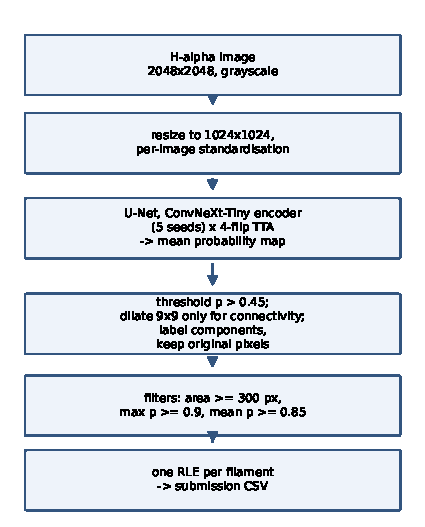
\includegraphics[width=0.78\columnwidth]{fig_pipeline.pdf}
\caption{End-to-end pipeline from a GONG image to the submission file.}
\label{fig:pipeline}
\end{figure}

\textbf{Data and targets.} The training set has 707 observations and 1154 annotated images (one to three annotators per observation, 8199 polygons); the test set has 180 images of $2048^2$ pixels. Polygons are rasterised with the pycocotools routine used by the scorer (\texttt{frPyObjects}); rasterising with \texttt{cv2.fillPoly} shifts edges by about a pixel. The target of an observation is the \emph{fraction of annotators} who marked each pixel, a soft map in $[0,1]$ downsampled to $1024^2$ by area interpolation. Annotators disagree strongly: one annotator's masks scored against another's give PQ $=0.345$ on the training set.

\textbf{Validation split.} Observations are sorted by capture time and cut into five contiguous blocks; block~2 (142 observations) is held out, so near-duplicate neighbouring observations never straddle the split, and all annotator versions of an observation stay together.

\textbf{Network and training.} A U-Net (\texttt{segmentation\_models\_pytorch}) with a ConvNeXt-Tiny encoder pre-trained on ImageNet (timm). The input is the grayscale image standardised per image and replicated to three channels. The loss is binary cross-entropy (positive weight 4) plus soft Dice against the soft target. We use AdamW, learning rate $3\!\times\!10^{-4}$ with a one-cycle schedule, batch size 4, mixed precision with gradient scaling and gradient clipping at norm 1, and random $640^2$ crops of the $1024^2$ image with rotation in $[-180^\circ,180^\circ]$, scale in $[0.8,1.25]$, flips and brightness/contrast jitter. Training takes about 53 minutes for 60 epochs on one NVIDIA T4. The final networks are trained on all training observations with different seeds (one for 60 epochs, the others for 80).

\textbf{Inference and post-processing.} Each network is applied to the full $1024^2$ image with four flips (identity, horizontal, vertical, both) and the probabilities are averaged over flips and over the five networks. The map is resized to $2048^2$ and processed as follows: (1) threshold at $p>0.45$; (2) dilate the mask with a $9\times9$ kernel \emph{only to decide connectivity}, so that fragments of one filament split by small gaps share a label; (3) label connected components on the dilated mask but keep only the original pixels of each; (4) discard components with fewer than 300 pixels, maximum probability below 0.9 or mean probability below 0.85. Each remaining component is one filament, encoded as a column-major RLE row. The parameters come from a grid search on validation PQ, and the eight best settings lie within 0.003 PQ of each other.

\begin{figure*}[t]
\centering
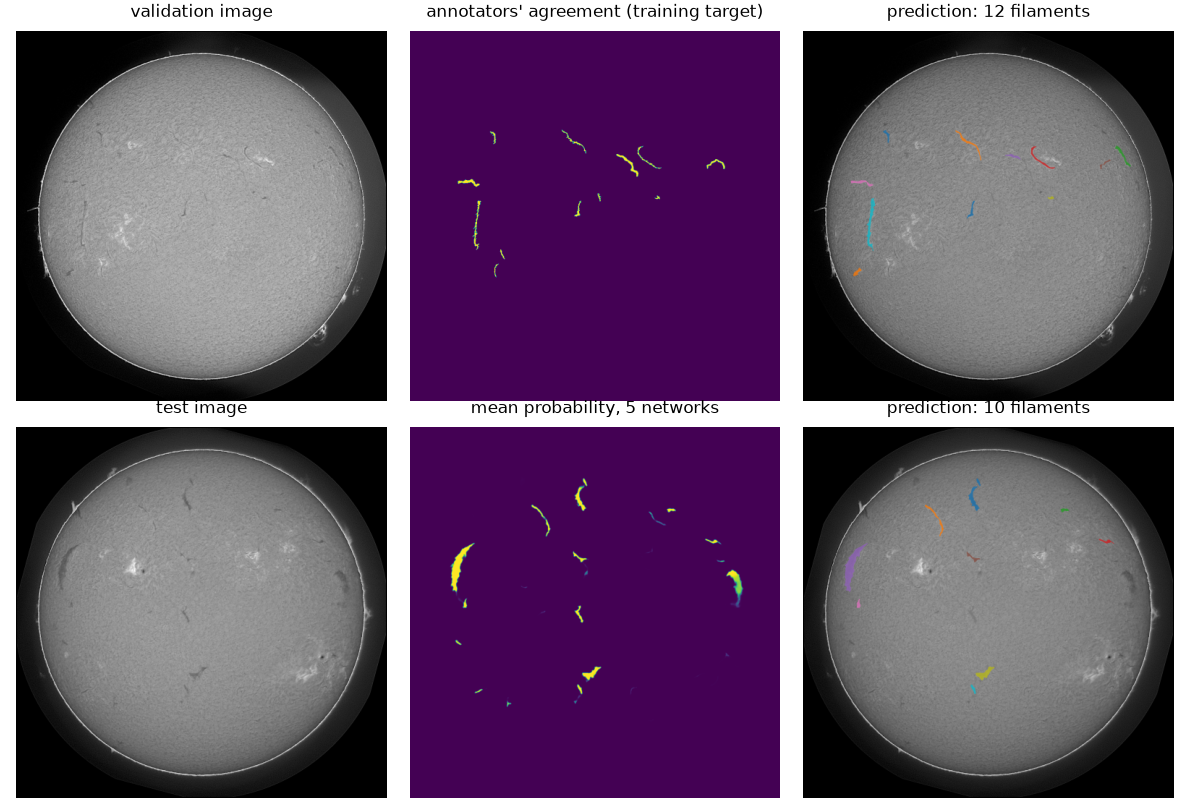
\includegraphics[width=0.82\textwidth]{fig_examples.png}
\caption{Top: a validation observation, the training target (annotator agreement) and our prediction with one colour per filament. Bottom: a test image, the mean probability of the five networks and the resulting filaments.}
\label{fig:examples}
\end{figure*}

% ==================================== %
% EVALUATION                           %
% ==================================== %
\section{Evaluation}
\textbf{Strategy.} PQ is the sum of IoU over matched pairs (IoU $>0.5$) divided by matches plus half the false positives and half the misses, pooled over every annotator's version of each held-out image; our scorer follows the organisers' self-evaluation notebook. We compare variants on the same split with one seed each. Because variants differ by little, we resample the 142 validation observations (2000 bootstrap draws) to get intervals.

\begin{table*}[t]
\centering\small
\begin{tabular}{lcc}
\hline
Variant (held-out block, PQ over all annotator images) & default & tuned\\
\hline
ResNet34 U-Net, 40 epochs (baseline) & 0.377 & 0.421\\
\quad + illumination flattening (divide by blurred image) & 0.373 & 0.415\\
\quad + majority-vote hard target & 0.362 & 0.414\\
\quad + Tversky loss ($\alpha{=}0.7$ on false positives) & 0.333 & 0.385\\
\quad at $1536^2$ resolution, $768^2$ crops & 0.374 & 0.421\\
ResNet34 U-Net, 80 epochs & 0.382 & 0.427\\
ResNet50 U-Net, 60 epochs & 0.382 & 0.422\\
\textbf{ConvNeXt-Tiny U-Net, 60 epochs} & \textbf{0.405} & \textbf{0.449}\\
Average of three ResNet34 variants / those plus the 80-epoch one & -- & 0.425 / 0.425\\
\hline
\multicolumn{3}{l}{Final post-processing (0.45, 9, 300, 0.9, mean 0.85), 95\% bootstrap interval:}\\
ConvNeXt-Tiny, 60 epochs & \multicolumn{2}{c}{\textbf{0.454} [0.439, 0.470]}\\
ResNet34, 80 epochs & \multicolumn{2}{c}{0.442 [0.427, 0.457]}\\
Paired difference ConvNeXt $-$ ResNet34 & \multicolumn{2}{c}{+0.012 [+0.004, +0.022]}\\
\hline
\end{tabular}
\caption{Single runs, one seed each. ``Default'' post-processing is (threshold 0.6, dilation 9, area $\ge50$); ``tuned'' is (0.5, 9, $\ge300$, max probability $\ge0.95$). The averaging row uses threshold 0.45 and maximum-probability filter 0.9. Intervals only reflect the sampling of observations, not seed-to-seed variation.}
\label{tab:exp}
\end{table*}

\textbf{Results.} (i) Post-processing gave the largest single jump: the first search raised the ResNet34 baseline from 0.377 to 0.421. (ii) The ConvNeXt-Tiny encoder gave a further +0.02 over the best ResNet34 with either post-processing, and the paired interval of its advantage excludes zero at the final settings; a larger ResNet (ResNet50) gave nothing. (iii) Higher resolution, illumination flattening and majority-vote targets did not improve over the baseline, and the Tversky loss was worse (it also shifts the calibration of the probabilities, so its default-parameter score is not a fair comparison, but it stayed behind after tuning). (iv) Averaging ConvNeXt-Tiny with a ResNet34 or ResNet50 network gave no gain on validation (0.451 and 0.450 against 0.452 for ConvNeXt-Tiny alone at an earlier post-processing setting); ConvNeXt-Small matched ConvNeXt-Tiny (0.454) and averaging the two gave +0.004, within noise, and since its fp16 weights exceed GitHub's 100~MB file limit it is not in the final ensemble. On the public leaderboard, averaging three ConvNeXt-Tiny seeds scored 0.39 against 0.37 for a single one, and three ResNet34 seeds scored 0.37 against 0.36 for one; five ConvNeXt-Tiny seeds also scored 0.39, so we saw no further gain beyond three. These differences are at or near the 0.01 resolution of the displayed score and use about half of the test images, and we could not validate seed averaging on our split because only one ConvNeXt-Tiny network was trained without the held-out block.

\textbf{Strengths and weaknesses.} The approach is simple and cheap: inference takes about three seconds per image and network on a 12-thread CPU, and every number here can be regenerated from the repository. Its weaknesses are the ones the numbers show. The post-processing was tuned on the same 142 observations used to report validation PQ, so those figures are optimistic, and the public score is lower (0.39 for the final ensemble). The reference is noisy (inter-annotator PQ 0.345, below our validation score, which says more about the labels than about human performance). A semantic model plus component analysis cannot separate touching filaments or reunite broken ones beyond the dilation heuristic, and barbs are limited by working at $1024^2$ (the one higher resolution we tried used a ResNet34 and did not help). Promising next steps are instance-aware heads, per-annotator modelling, and seed-level validation of the ensemble.

\textbf{Reproducibility.} The repository (\url{https://github.com/MattBuiles/filament-segmentation-2026}) contains the training and post-processing code, an exact PQ scorer, fp16 weights of the final networks, an executed notebook, and \texttt{predict.py}, which regenerates the submission from the weights. On CPU with fp16 weights it reproduces the submitted filaments with mean mask IoU above 0.999.
